 
\documentclass[10pt,a4paper]{article}
\usepackage[utf8]{inputenc}
\usepackage[spanish]{babel}
\usepackage{amsmath}
\usepackage{amsfonts}
\usepackage{amssymb}
\usepackage{graphicx}
\usepackage{natbib}
\usepackage{lineno}
\usepackage{ragged2e}
\usepackage{multicol}
\setlength\columnsep{38pt}
\usepackage{enumerate} 
\usepackage[left=1.94cm,top=1.59cm,right=1.9cm,bottom=0.59cm]{geometry} 
\usepackage{fancyhdr}
\usepackage{url}

\begin{document}
		
		\begin{center}
			\huge \textbf{Balance ScoreCard y Business Model Canvas} 
		\end{center}
		\vspace{\baselineskip}
		\begin{center}
			
\includegraphics[scale=0.37]{./Imagenes/logo}
		\end{center}
		\vspace{\baselineskip}
		\begin{multicols}{2}
			\small
			\begin{center}
				Nelia Escalante Marón\\
				2014049551\\
				UPT – Ingeniería de Sistemas\\
				EPIS\\
				Tacna, Perú\\
				\vspace{\baselineskip}
				Yerson Coaquira Calizaya\\
				2015053225\\
				UPT – Ingeniería de Sistemas\\  
				EPIS\\
				Tacna, Perú\\                 
				\vspace{\baselineskip}
				Flor Condori Gutierrez\\
				2015053227\\
				UPT – Ingeniería de Sistemas\\  
				EPIS\\	
				Tacna, Perú\\                 
				\columnbreak
				
				\vspace{\baselineskip}
				Christian Cespedes Medina\\
				2010036256\\
				UPT – Ingeniería de Sistemas\\  
				EPIS\\	
				Tacna, Perú\\                 

				\vspace{\baselineskip}
				Javier Octavio Arteaga Ramos \\
				2007028981\\
				UPT – Ingeniería de Sistemas\\  
				EPIS\\	
				Tacna, Perú\\                 

			\end{center}
			\normalsize			
		\end{multicols}
		\vspace{\baselineskip}
	
		\rule{167mm}{0.1mm}\\
		
		\textbf{\textit{\large Abstract}}\rule[1.5mm]{5mm}{0.1mm} El Balanced Scorecard (BSC) y el modelo Canvas pueden enlazarse como herramientas complementarias para los emprendedores. La primera desarrolla objetivos y medidas operativas en cuatro perspectivas principales para alcanzar la misión y estrategia. La segunda ha supuesto una revolución en la generación de modelos de negocio, estableciendo nueve apartados que reflejan su lógica. En el artículo se desarrolla un modelo de trabajo que, partiendo de la necesidad de disponer de un BSC, relaciona su diseño con la información recogida previamente en el modelo Canvas, señalando su mutua necesida\\
		
		\textit{The Balanced Scorecard (BSC) and the Canvas model can be linked as complementary tools for entrepreneurs. The first develops objectives and operational measures in four main perspectives to achieve the mission and strategy. The second one has supposed a (re-) evolution in the generation of business models, establishing nine sections that reflect its logic. The article develops a work model that, starting from the need to have a BSC, relates its design with the information previously collected in the Canvas model, pointing out their mutual need.}
				
		\vspace{\baselineskip}
		
		\textbf{\textit{\large Keybwords}}\rule[1.5mm]{5mm}{0.1mm} BMC, Web 2.0, Bsc y Bmc en los negocios, cloud
						
		\rule{167mm}{0.1mm}
		
		\vspace{\baselineskip}
		
		\begin{center}
			\textbf{INTRODUCCIÓN}
		\end{center}
		
		
		
		Balanced Scorecard y Business model canvas son técnicas de análisis empresarial . Ambas técnicas son útiles para mejorar el desempeño organizacional. Pero sus aplicaciones difieren. Ambos se pueden usar junto con los indicadores clave de rendimiento para monitorear y mejorar el rendimiento de la organización.\\
		
		De acuerdo con el informe Global Entrepreneurship Monitor (GEM) del año 2012, son necesarios más esfuerzos para consolidar las nuevas empresas. Se reconoce ampliamente que su desarrollo y supervivencia no depende tanto de tener una buena idea de negocio sino de su adecuada ejecución y gestión. En este sentido, desde diferentes ámbitos se defiende que los emprendedores/as necesitan herramientas que les permitan desarrollar sus estrategias y les indiquen el grado de consecución de sus objetivos y actividades como medio de incrementar su probabilidad de supervivencia (Davila \& Oyon, 2009).\\
		
		Por consiguiente, se propone que el diseño del BSC facilita traducir las ideas desarrolladas en el Canvas en objetivos, factores claves de éxito, e indicadores que facilitan la correcta implantación de la estrategia deseada. Argumentamos que el BSC se ayuda del Canvas y lo completa para facilitar una estructura sobre la que desarrollar la estrategia, e invitamos a los emprendedores a desarrollar el BSC como una continuidad de su modelo de negocio Canvas, facilitando su implantación y gestión. Para ello, junto a la consideración de trabajos teóricos y empíricos que se han ocupado de este tema, incorporamos algunas de las conclusiones que hemos alcanzado a través de nuestro contacto directo con emprendedores, en reuniones de formación y asesoramiento, así como en clases de posgrado especializadas.
		
		\vspace{\baselineskip}
		
		\begin{center}
			\textbf{MARCO TEÓRICO}
		\end{center}
			
		\section{Balanced ScoreCard (BSC)}	
		
		En 1992, Kaplan y Norton de Harvard University revolucionaron la administración de empresas al introducir un concepto bastante efectivo para alinear la empresa hacia la consecución de las estrategias del negocio, a través de objetivos e indicadores tangibles.\\
		\\		
		Puede entenderse al BSC como una herramienta o metodología, lo importante es que convierte la visión en acción mediante un conjunto coherente de indicadores agrupados en 4 categorías de negocio.\\
		\\
		Según Mario Vogel, \textit{"BSC lo ayuda a balancear, de una forma integrada y estratégica, el progreso actual y suministra la dirección futura de su empresa, para ayudarle a convertir la visión en acción por medio de un conjunto coherente de indicadores, agrupados en 4 diferentes perspectivas, a través de las cuales se puede ver el negocio en su totalidad."}\\
		\\
		Las 4 categorías de negocio son: Financieras, Clientes, Procesos Internos y Formación y Crecimiento. BSC sugiere que estas perspectivas abarcan todos los procesos necesarios para el correcto funcionamiento de una empresa y deben ser considerados en la definición de los indicadores. De acuerdo a las características propias de cada negocio pueden existir incluso más, pero difícilmente habrá menos de las mencionadas.\\
		\\
		El equilibrio entre los indicadores es lo que da nombre a la metodología, pues se presenta un balance entre los externos relacionados con accionistas y clientes, y los internos de los procesos, capacitación, innovación y crecimiento; también existe un equilibrio entre indicadores de resultados, los cuales ven los esfuerzos (principalmente económicos) pasados e indicadores que impulsan la acción futura (capacitación, innovación, aprendizaje, etc.).[\cite{herrera2015modelo}]
		
			\subsection{Beneficios}
			
			El Balanced Scorecard induce una serie de resultados que favorecen la administración de la compañía, pero para lograrlo es necesario implementar la metodología y la aplicación para monitorear, y analizar los indicadores obtenidos del análisis. Entre otros podemos considerar las siguientes ventajas:
			
			\begin{itemize}
				\item Alineación de los empleados hacia la visión de la empresa.
				\item Comunicación hacia todo el personal de los objetivos y su cumplimiento.
				\item Redefinición de la estrategia en base a resultados.
				\item Traducción de la visión y estrategias en acción.
				\item Favorece en el presente la creación de valor futuro
				\item Integración de información de diversas áreas de negocio.
				\item Capacidad de análisis.
				\item Mejoría en los indicadores financieros.
				\item Desarrollo laboral de los promotores del proyecto.
			\end{itemize}
		
			\subsection{Perspectivas del Balanced ScoreCard}
			
			A pesar de que son 4 las perspectivas que tradicionalmente identifican un BSC, no es indispensable que estén todas ellas; estas perspectivas son las más comunes y pueden adaptarse a la gran mayoría de las empresas, y no constituyen una condición indispensable para construir un modelo de negocios.
			
			\begin{itemize}
				\item Perspectiva financiera
				
				Históricamente los indicadores financieros han sido los más utilizados, pues son el reflejo de lo que está ocurriendo con las inversiones y el valor añadido económico, de hecho, todas las medidas que forman parte de la relación causa-efecto, culminan en la mejor actuación financiera.
				
				\item Perspectiva del cliente
				
				Como parte de un modelo de negocios, se identifica el mercado y el cliente hacia el cual se dirige el servicio o producto. La perspectiva del cliente es un reflejo del mercado en el cual se está compitiendo. Brinda información importante para generar, adquirir, retener y satisfacer a los clientes, obtener cuota de mercado, rentabilidad, etc. Kaplan \& Norton afirman: \textit{"La perspectiva del cliente permite a los directivos de unidades de negocio articular la estrategia de cliente basada en el mercado, que proporcionará unos rendimientos financieros futuros de categoría superior."} 
				 
				\item Perspectiva procesos internos
				
				Para alcanzar los objetivos de clientes y financieros es necesario realizar con excelencia ciertos procesos que dan vida a la empresa. Esos procesos en los que se debe ser excelente son los que identifican los directivos y ponen especial atención para que se lleven a cabo de una forma perfecta, y así influyan a conseguir los objetivos de accionistas y clientes.
				
				\item Perspectiva de formación y crecimiento.
				
				Es la perspectiva donde más tiene que ponerse atención, sobre todo si piensan obtenerse resultados constantes a largo plazo. Aquí se identifica la infraestructura necesaria para crear valor a largo plazo. Hay que lograr formación y crecimiento en 3 áreas: personas, sistemas y clima organizacional. 
				
			\end{itemize}
			[\cite{osterwalder2014canvas}]
		
			\subsection{Uso de Balanced ScoreCard}
			
			La filosofía principal para sugerir perspectivas de indicadores es que todos ellos, en perfecto balance, abarcan casi la totalidad de los indicadores necesarios para monitorear la empresa, pero la pregunta es cómo vincular las distintas perspectivas[\cite{baraybar2011cuadro}]\\
			\\
			Todo lo que pasa en cualquier empresa es un conjunto de hipótesis sobre la causa y efecto entre indicadores. Cualquier acción que se ejecute, tendrá un impacto directo sobre otra variable, es por eso que la perspectiva de Formación y Crecimiento es la base que permite crear la infraestructura necesaria para crecer en las otras perspectivas. Lo importante es saber que ninguna perspectiva funciona en forma independiente, sino que puede iniciarse una acción con alguna de ellas y repercutirá sobre todas las demás.\\
			\\
			Un ejemplo simple puede ilustrar esta situación: Supongamos que los empleados necesitan capacitación e instalaciones adecuadas para estar satisfechos y, por extensión, realizar bien su trabajo; si realizan bien su trabajo de forma individual estarán realizando procesos de negocio complejos que afectarán directamente el producto o servicio ofrecido para que éste sea de mejor calidad; un buen servicio provocará que el cliente esté satisfecho, recomiende y, por extensión, incremente la cuota de mercado, lo cual a su vez repercutirá en mayores ingresos y rentabilidad. [\cite{fernandez2001balanced}]\\
			\\
			Pareciera un ejemplo muy trivial, pero de alguna forma es como afectan ciertas perspectivas sobre todas las demás. Cada una de las medidas forma parte de la cadena de relaciones causa-efecto que dan significado a la estrategia en la unidad de negocio.
			
			\subsection{Etapas de implementación  de un Balance ScoreCard}
			
			Primero, implementación de sistemas corporativos confiables y estandarizados para la generación de indicadores como: ERPs, CRMs, BPMs y/o BPCs.\\
			\\
			Segundo, definición del plan estratégico, visión, perspectivas, estrategias, metas, objetivos e indicadores de desempeño.\\
			\\
			Tercero, selección de los indicadores de desempeño clave (KPIs), provenientes de los sistemas corporativos, y en su defecto, implementación de nuevos controles internos o flujos de trabajo para su obtención.\\
			\\
			Cuarto, generación de tableros de control conectados directamente a las fuentes estandarizadas de información.
		
		\newpage
		
		\section{Business Model Canvas (BMC)}
		
		El Business Model Canvas, método ideado por Alex Osterwalder, es una herramienta que permite obtener una visión de todos los elementos de la actividad empresarial en un único lienzo canvas. Una metodología para definir nuevos modelos de negocio o ayudar a nuevas empresas a integrarse en modelos de negocio de éxito ya establecidos por otras compañías o crear negocios novedosos.\\
		\\
		El lienzo de modelos de Negocio es extensamente utilizado por las startups, debido a la flexibilidad y sencillez que ofrece a la hora de trabajar. Consiste en responder a una serie de preguntas clave y distribuir todos los elementos que pueden intervenir en la actividad de la empresa de forma ordenada en un esquema estructurado por 9 bloques.
		
		\begin{center}
			
\includegraphics[scale=1]{./Imagenes/img01}
		\end{center}
	
			\subsection{Componentes de Business Model Canvas}
			\vspace{\baselineskip}
				\subsubsection{Segmento de clientes}				
				Para analizar este bloque existen lienzos de trabajo específicos como el lienzo de propuesta de valor, el lienzo de persona o los conocidos mapas de empatía. 
				
				\subsubsection{Propuesta de Valor}				
				Para definir tu propuesta de valor es crítico saber qué problema ayudas a solucionar a tus clientes. 
				
				\subsubsection{Canales}				
				Identifica cuál va a ser el medio por el que vas a hacer llegar tu propuesta de valor a tu segmento de clientes objetivo. A veces tu estrategia de Marketing online será clave en este apartado y otras menos. 
				
				\subsubsection{Relación con clientes}
				Reflexiona sobre cuál va a ser tu relación con los clientes. Dónde empieza y dónde acaba esta relación. También tu estrategia en Redes Sociales y en Marketing online será clave en tu relación con clientes. 
				
				\subsubsection{Flujo de ingresos}
				Tienes que tener claro cómo vas a ganar dinero. Al principio pon todas las opciones que se te ocurran y posteriormente testa cómo y cuánto está dispuesto a pagar tu cliente objetivo (venta de activos, suscripción, publicidad…)
				
				\subsubsection{Recursos Clave}
				¿Qué necesitas para llevar a cabo la actividad de tu empresa? Los recursos pueden ser físicos, económicos, humanos o intelectuales. 
				
				\subsubsection{Actividades Clave}
				Cuáles son las actividades nucleares para tu empresa. Es importante tener claro este bloque porque es a lo que se dedicará tu empresa, el resto, lo que aporta menos valor, podrás subcontratarlo. 
				
				\subsubsection{Asociaciones Clave}
				Enumera los agentes con los que necesitas trabajar para hacer posible el funcionamiento del modelo de negocio (alianzas estratégicas, proveedores…) 
\subsubsection{Estructura de Costes}
				Después de analizar las actividades clave, los recursos clave y asociaciones clave, reflexiona sobre los costes que tiene tu empresa. 
				
			\begin{center}
				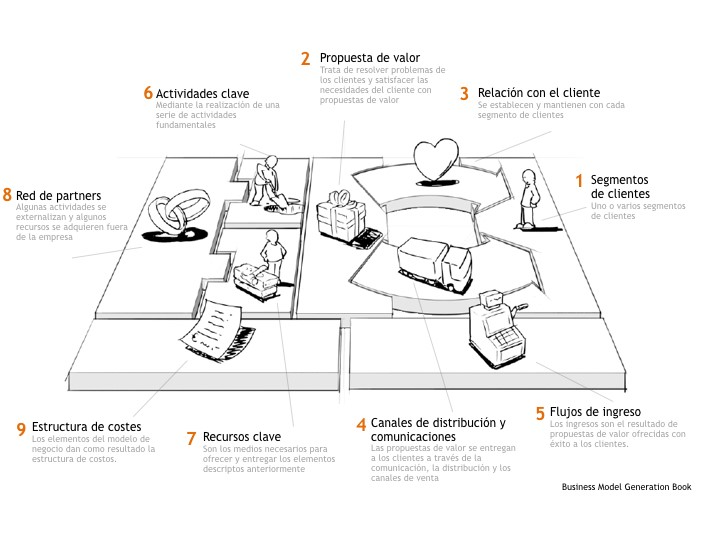
\includegraphics[scale=0.6]{./Imagenes/img02}
			\end{center}
			
		\subsection{Ventajas y Desventajas del BMC}
		
		\begin{center}
			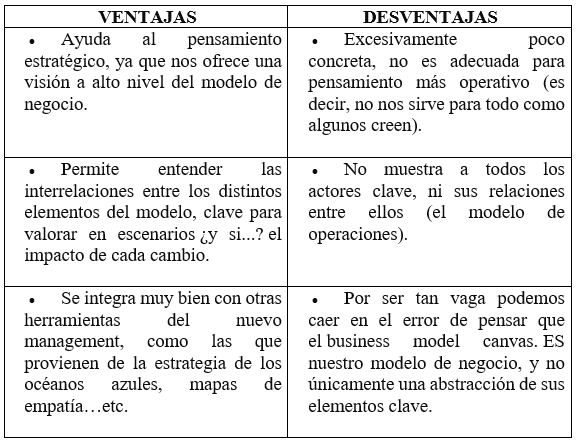
\includegraphics[scale=0.65]{./Imagenes/img03}
		\end{center}
	
		\subsection{EJEMPLO: Caso de estudio del Business Model Canvas}
		
		Posiblemente la mejor forma de comprender algo es con un ejemplo, así que he decidido utilizar como caso de estudio uno de los negocios considerados como más innovadores para la ocasión: NESPRESSO
				
				
			
\end{document}}